\documentclass[12pt]{article}
\usepackage[table]{xcolor}
\usepackage[shortlabels]{enumitem}
\usepackage{tabularx,xltabular}
\usepackage{graphicx}
\usepackage{hyperref}
\usepackage{verbatim}
\usepackage{geometry}
\usepackage{ulem}
\usepackage[official]{eurosym}
\usepackage{tikz}
\usetikzlibrary{arrows,backgrounds,calc,decorations.markings,patterns,3d,positioning,fit,angles, quotes}
\usepackage{pgfplots}
\pgfplotsset{compat = newest}
\usetikzlibrary{fit}
\newcommand\addvmargin[1]{
\usetikzlibrary{arrows}
\node[fit=(current bounding box),inner ysep=#1,inner xsep=0]{};}
\usepackage{cancel}
\usepackage{fontspec}
\usepackage{array}  
\geometry{a4paper, top=2cm, left=2cm, right=2cm, bottom=2cm, headsep=1cm}
\usepackage{tabu}
\usepackage{pst-node}
\usepackage{colortbl}
\usepackage{array}
\usepackage{german}
\setlength\parindent{0pt}
\newcolumntype{?}{!{\vrule width 1pt}}
\usepackage{makecell}
\usepackage{pbox}
\usepackage{amssymb}
\usepackage{amsmath}
\usepackage{booktabs}
\newcolumntype{L}[1]{>{\raggedright\let\newline\\\arraybackslash\hspace{0pt}}m{#1}}
\newcolumntype{C}[1]{>{\centering\let\newline\\\arraybackslash\hspace{0pt}}m{#1}}
\newcolumntype{R}[1]{>{\raggedleft\let\newline\\\arraybackslash\hspace{0pt}}m{#1}}
\begin{document}
\rightline{}
\centerline{{\Large }} 
\vspace{1cm}
\noindent \\


\begin{tabularx}{\textwidth}{|C{1.0cm}|X|}
\arrayrulecolor{black}\hline
a)&{\begingroup\setlength{\jot}{-0.03cm}
\tikzstyle{background grid}=[draw, black!15,step=.5cm]
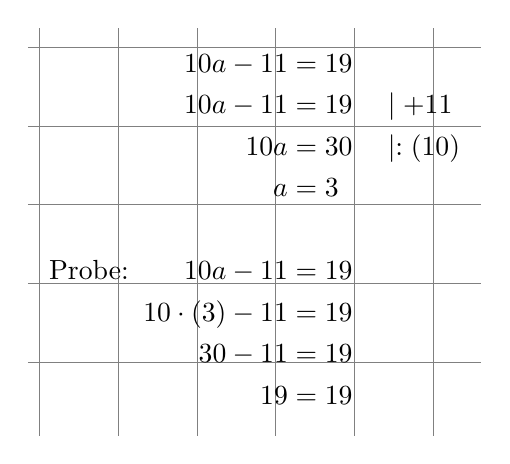
\begin{tikzpicture}[show background grid]
\node[below right] at (0,0.1) {
$\begin{aligned}
10a-11 &=19& &  \\
10a - 11 &=19& & \mid + 11\\
10a &=30& & \mid :\left(10\right)\\
a &=3& & 
\\
\\
\mbox{Probe:}\qquad 10a-11 &=19& &  \\
10\cdot \left(3\right)-11 &=19& &  \\
30-11 &=19& &  \\
19 &=19& &  \\
\end{aligned}$};
\end{tikzpicture}
\endgroup}
\\\hline
\end{tabularx}
\vspace{0.5cm}
\begin{tabularx}{\textwidth}{|C{1.0cm}|X|}
\arrayrulecolor{black}\hline
a)&{\begingroup\setlength{\jot}{-0.03cm}
\tikzstyle{background grid}=[draw, black!15,step=.5cm]
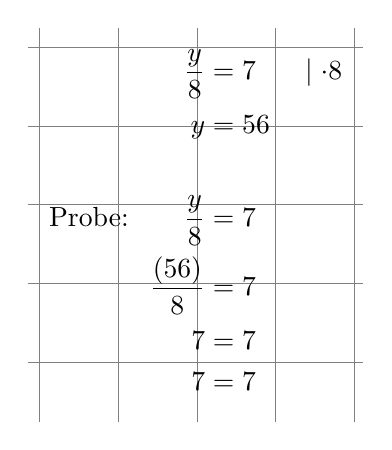
\begin{tikzpicture}[show background grid]
\node[below right] at (0,0.1) {
$\begin{aligned}
{{\frac{y}{8}}} &=7& & \mid \cdot 8\\
y &=56& & 
\\
\\
\mbox{Probe:}\qquad {{\frac{y}{8}}} &=7& &  \\
{{\frac{\left(56\right)}{8}}} &=7& &  \\
7 &=7& &  \\
7 &=7& &  \\
\end{aligned}$};
\end{tikzpicture}
\endgroup}
\\\hline
\end{tabularx}
\vspace{0.5cm}
\begin{tabularx}{\textwidth}{|C{1.0cm}|X|}
\arrayrulecolor{black}\hline
a)&{\begingroup\setlength{\jot}{-0.03cm}
\tikzstyle{background grid}=[draw, black!15,step=.5cm]
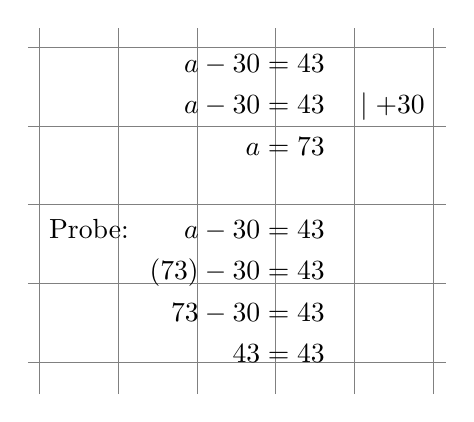
\begin{tikzpicture}[show background grid]
\node[below right] at (0,0.1) {
$\begin{aligned}
a-30  &= 43& &  \\
a - 30 &=43& & \mid + 30\\
a &=73& & 
\\
\\
\mbox{Probe:}\qquad a-30  &= 43& &  \\
\left(73\right)-30  &= 43& &  \\
73-30 &=43& &  \\
43 &=43& &  \\
\end{aligned}$};
\end{tikzpicture}
\endgroup}
\\\hline
\end{tabularx}
\vspace{0.5cm}
\begin{tabularx}{\textwidth}{|C{1.0cm}|X|}
\arrayrulecolor{black}\hline
a)&{\pbox{5cm}{
$\begin{aligned}
geg.: g&=2,3 cm \\
   h&=3,3 cm \\
ges.: A&=? \\
A&=\frac{g \cdot h}{2} \\
&=2,3 \cdot \frac{3,3}{2}\\
\makebox[0pt][l]{\uuline{\phantom{$A=3,79~cm^2$} } }
A&=3,79~cm^2
\end{aligned}$
\tikzstyle{background grid}=[draw, black!15,step=.5cm]
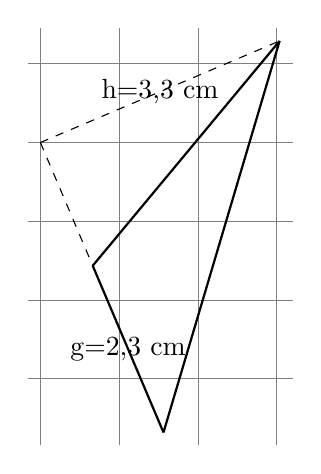
\begin{tikzpicture}[show background grid]
\draw[thick,black] (293:1.7000000000000002) -- node{g=2,3 cm} (293:4.0);
\draw[thick,black] (293:1.7000000000000002)  -- (383:3.3);
\draw[thick,black] (293:4.0)  -- (383:3.3);
\draw[dashed,black] (0,0)  -- node{h=3,3 cm} (383:3.3);
\draw[dashed,black] (0,0)  -- (293:1.7000000000000002);
\end{tikzpicture}
}}
\\\hline
\end{tabularx}
\vspace{0.5cm}
\begin{tabularx}{\textwidth}{|C{1.0cm}|X|}
\arrayrulecolor{black}\hline
a)&{\pbox{5cm}{
\tikzstyle{background grid}=[draw, black!15,step=.5cm]
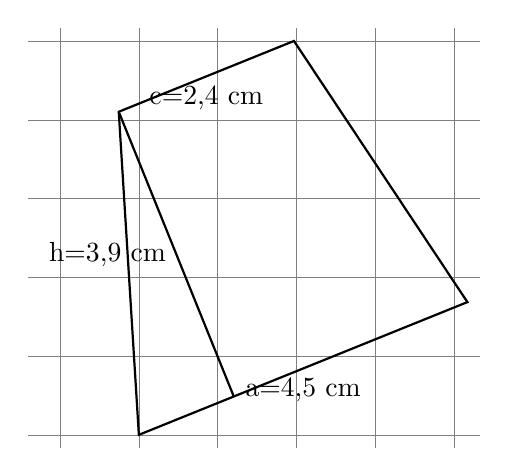
\begin{tikzpicture}[show background grid]
\draw[thick,black,rotate=22] (0,0) -- node[below]{a=4,5 cm} ++(4.5,0) -- ++(-0.8,3.9) --node[below]{c=2,4 cm} ++(-2.4,0) --cycle;
\draw[thick,black,rotate=22] (1.3,0) --node[left]{h=3,9 cm}  ++(0,3.9);
\end{tikzpicture}
$\begin{aligned}
geg.: a&=4,5 cm \\
   c&=2,4 cm \\
   h&=3,9 cm \\
ges.: A&=? \\
A&=\frac{a+c}{2}\cdot h \\
&=\frac{4,5+2,4}{2}\cdot3,9\\
\makebox[0pt][l]{\uuline{\phantom{$A=13,46~cm^2$} } }
A&=13,46~cm^2
\end{aligned}$
}}
\\\hline
\end{tabularx}
\vspace{0.5cm}
\begin{tabularx}{\textwidth}{|C{1.0cm}|X|}
\arrayrulecolor{black}\hline
a)&{\pbox{5cm}{
$\begin{aligned}
geg.: g&=3,9 cm \\
   h&=2,8 cm \\
ges.: A&=? \\
A&=g\cdot h \\
&=3,9\cdot 2,8 \\
\makebox[0pt][l]{\uuline{\phantom{$A=10,92~cm^2$} } }
A&=10,92~cm^2
\end{aligned}$
\tikzstyle{background grid}=[draw, black!15,step=.5cm]
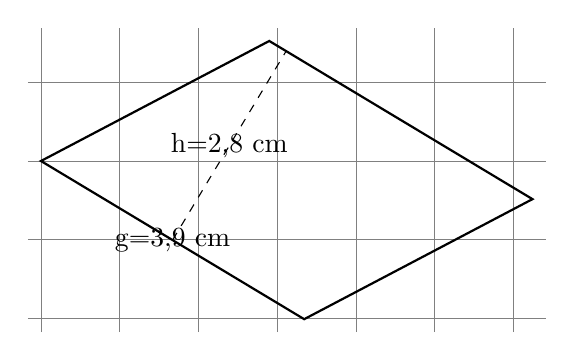
\begin{tikzpicture}[show background grid]
\draw[thick,black,rotate=329] (0,0) -- node{g=3,9 cm} ++(3.9,0) -- ++(1.7,2.8) -- ++(-3.9,0) --cycle;
\draw[dashed,black,rotate=329] (1.95,0)  -- node{h=2,8 cm} ++(0,2.8);
\end{tikzpicture}
}}
\\\hline
\end{tabularx}
\vspace{0.5cm}
\begin{tabularx}{\textwidth}{|C{1.0cm}|X|}
\arrayrulecolor{black}\hline
a)&{\pbox{6cm}{$U=2\cdot a+2\cdot b$ \\ $U=2\cdot1cm+2\cdot3cm=8cm$ \\$A=a\cdot b$ \\ $A=1\cdot3=3cm^2$ \\\tikzstyle{background grid}=[draw, black!15,step=.5cm]
\noindent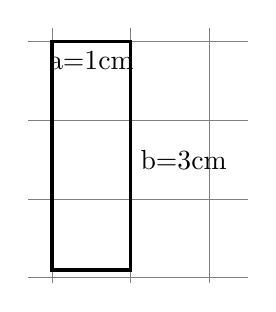
\begin{tikzpicture}[show background grid]
\draw[black, very thick] (0cm,0.1cm) rectangle (1cm,3cm);
\draw (0.5cm,3cm) node[below]{a=1cm}; 
\draw (1cm,1.5cm) node[right]{b=3cm}; 
\end{tikzpicture}}}
\\\hline
\end{tabularx}
\vspace{0.5cm}
\begin{tabularx}{\textwidth}{|C{1.0cm}|X|}
\arrayrulecolor{black}\hline
a)&{$\begin{aligned}
\textcolor{red}{a=9} & \rightarrow\\
3 \cdot a + 4 \cdot a=&3 \cdot \textcolor{red}{9} + 4 \cdot \textcolor{red}{9}=63\\
\end{aligned}$}
\\\hline
\end{tabularx}
\vspace{0.5cm}
\begin{tabularx}{\textwidth}{|C{1.0cm}|X|}
\arrayrulecolor{black}\hline
b)&{$\begin{aligned}
\textcolor{red}{a=-1} & \rightarrow\\
2 \cdot a + 4 \cdot a=&2 \cdot \textcolor{red}{(-1)} + 4 \cdot \textcolor{red}{(-1)}=-6\\
\end{aligned}$}
\\\hline
\end{tabularx}
\vspace{0.5cm}
\begin{tabularx}{\textwidth}{|C{1.0cm}|X|}
\arrayrulecolor{black}\hline
a)&{$2 + 3 - 1=4$}
\\\hline
\end{tabularx}
\vspace{0.5cm}
\begin{tabularx}{\textwidth}{|C{1.0cm}|X|}
\arrayrulecolor{black}\hline
b)&{$4 + 2 + x - 4x=6 - 3x$}
\\\hline
\end{tabularx}
\vspace{0.5cm}
\begin{tabularx}{\textwidth}{|C{1.0cm}|X|}
\arrayrulecolor{black}\hline
a)&{\tikzstyle{background grid}=[draw, black!15,step=.5cm]
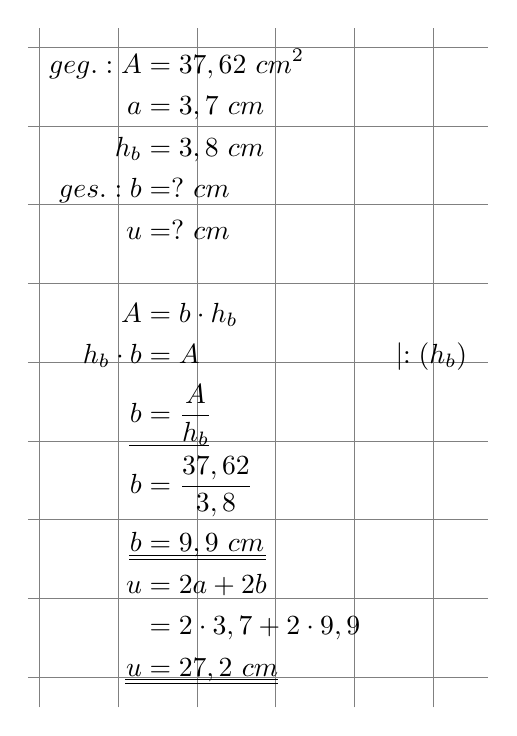
\begin{tikzpicture}[show background grid]
\node[below right] at (0,0.1) {
$\begin{aligned}
geg.: A &=37,62~cm^2& & \\
  a &=3,7~cm& & \\
  h_b &=3,8~cm& & \\
ges.: b &=?~cm& & \\
u &=?~cm& & \\
& & & \\
A &=b\cdot h_b& & \\
h_b\cdot b &=A& & \mid :(h_b)\\
\makebox(0pt,-0.25cm)[l]{\uline{\phantom{$b ={{\frac{A}{h_b}}}  \\$}}}
b &={{\frac{A}{h_b}}}& & \\
b&=\frac{37,62}{3,8}& & \\
\makebox[0pt][l]{\uuline{\phantom{$b=9,9~cm  \\$}}}
b&=9,9~cm& & \\
u&=2a+2b & & \\
&=2\cdot3,7+2\cdot9,9& & \\
\makebox[0pt][l]{\uuline{\phantom{$u=27,2~cm     \\$}}}
u&=27,2~cm   & & \\
\end{aligned}$};
\end{tikzpicture}}
\\\hline
\end{tabularx}
\vspace{0.5cm}
\begin{tabularx}{\textwidth}{|C{1.0cm}|X|}
\arrayrulecolor{black}\hline
b)&{\tikzstyle{background grid}=[draw, black!15,step=.5cm]
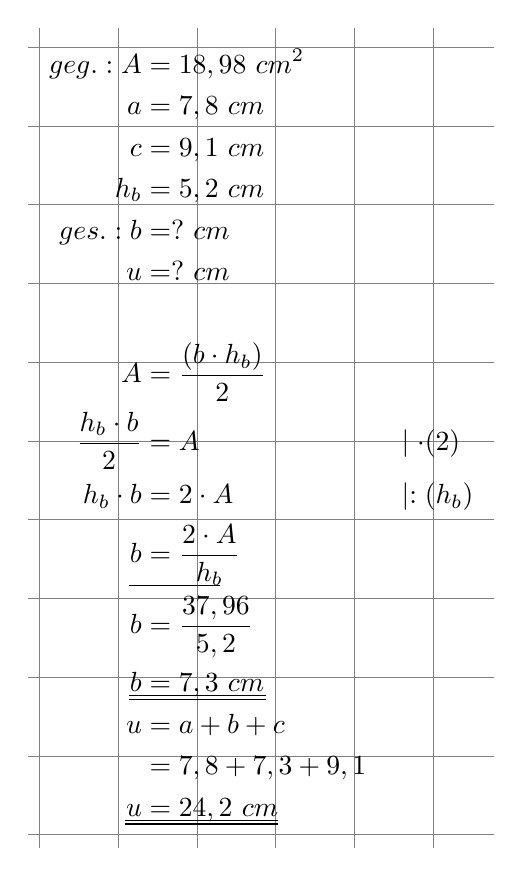
\begin{tikzpicture}[show background grid]
\node[below right] at (0,0.1) {
$\begin{aligned}
geg.: A &=18,98~cm^2& & \\
  a &=7,8~cm& & \\
  c &=9,1~cm& & \\
  h_b &=5,2~cm& & \\
ges.: b &=?~cm& & \\
u &=?~cm& & \\
& & & \\
A &={{\frac{\left(b\cdot h_b\right)}{2}}}& & \\
{{\frac{h_b\cdot b}{2}}} &=A& & \mid \cdot (2)\\
h_b\cdot b &=2\cdot A& & \mid :(h_b)\\
\makebox(0pt,-0.25cm)[l]{\uline{\phantom{$b ={{\frac{2\cdot A}{h_b}}}  \\$}}}
b &={{\frac{2\cdot A}{h_b}}}& & \\
b&=\frac{37,96}{5,2}& & \\
\makebox[0pt][l]{\uuline{\phantom{$b=7,3~cm  \\$}}}
b&=7,3~cm& & \\
u&=a+b+c& & \\
&=7,8+7,3+9,1& & \\
\makebox[0pt][l]{\uuline{\phantom{$u=24,2~cm     \\$}}}
u&=24,2~cm   & & \\
\end{aligned}$};
\end{tikzpicture}}
\\\hline
\end{tabularx}
\vspace{0.5cm}
\begin{tabularx}{\textwidth}{|C{1.0cm}|X|}
\arrayrulecolor{black}\hline
\end{tabularx}
\vspace{0.5cm}
\end{document}